



\chapter{Combinational Circuit}


\section{Review of Combinational Circuit}

In this section, we review fundamental concepts on digital circuit and logic desing, and mainly the one encountered in \verb|HLS|. \\


\subsection{Combinational Circuit}

$\mathrm{1}^\mathrm{st}$, recall that a combinational circuit are circuit in which \tbi{outputs depends only in current states of the input}, therefore any change in input affect the output after some delay.

Also, a combinational circuit doesn't have or use any memory or storage device. \autoref{fig:combinational_circuit:app_comb_circuit} presents applications of combinational circuit.


\subsection{Logic Gates}

\todo{Logic Gates} \uti{Logic Gates}

\begin{itemize}

\item \textit{Source: Section 6 video 39}

\item \textit{Contains some nice picture, maybe to insert them later in my summary report}

\end{itemize}


\newpage
\begin{figure}[h]
\centering
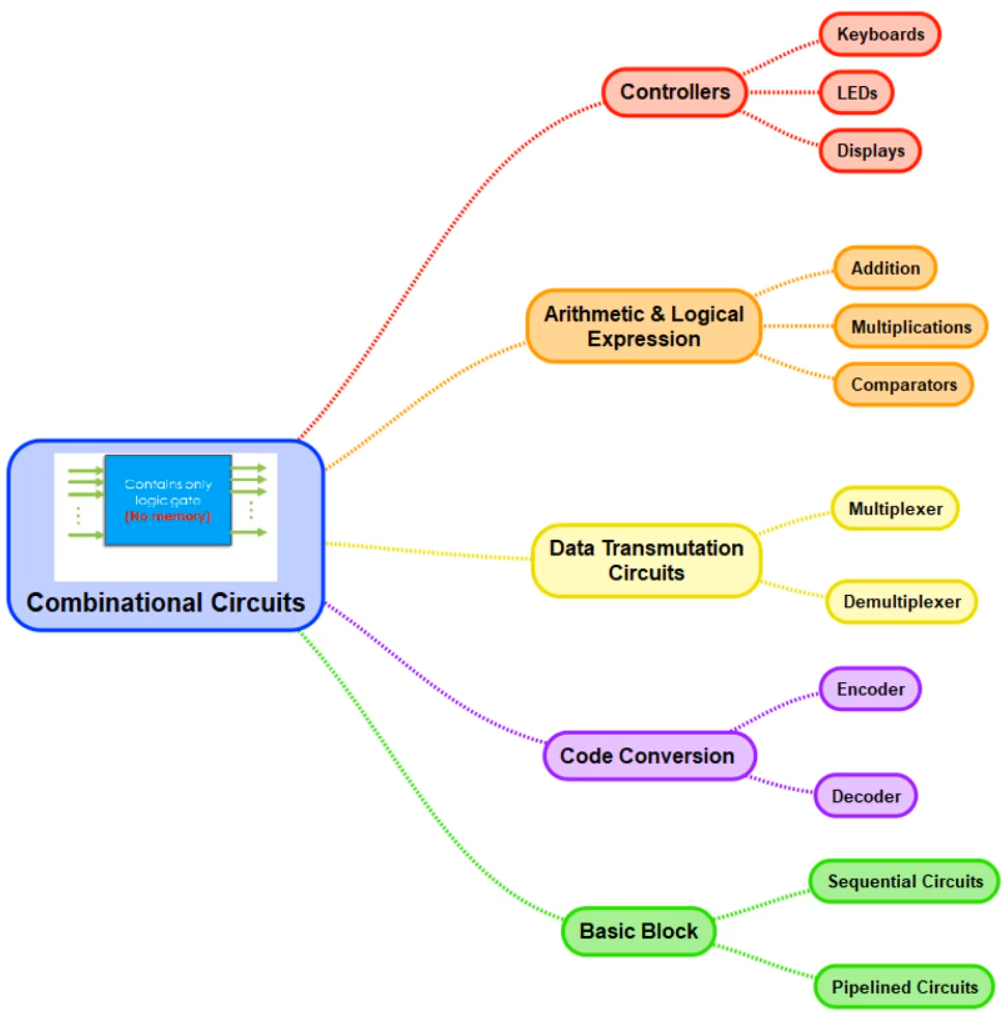
\includegraphics[scale=0.45,frame]{Figures/combinational_circuit/app_comb_circuit}
\caption{Combinatial Circuit Applications}
\label{fig:combinational_circuit:app_comb_circuit}
\end{figure}

\newpage
\section{Propagation Delay}
\label{sec:prop_delay}

Logic gates doesn't react to input instantly, it takes some time in order correct output is computed. In \autoref{fig:combinational_circuit:delay_gate_example}, an example of NAND gate delay is shown.


\begin{figure}[h]
\centering
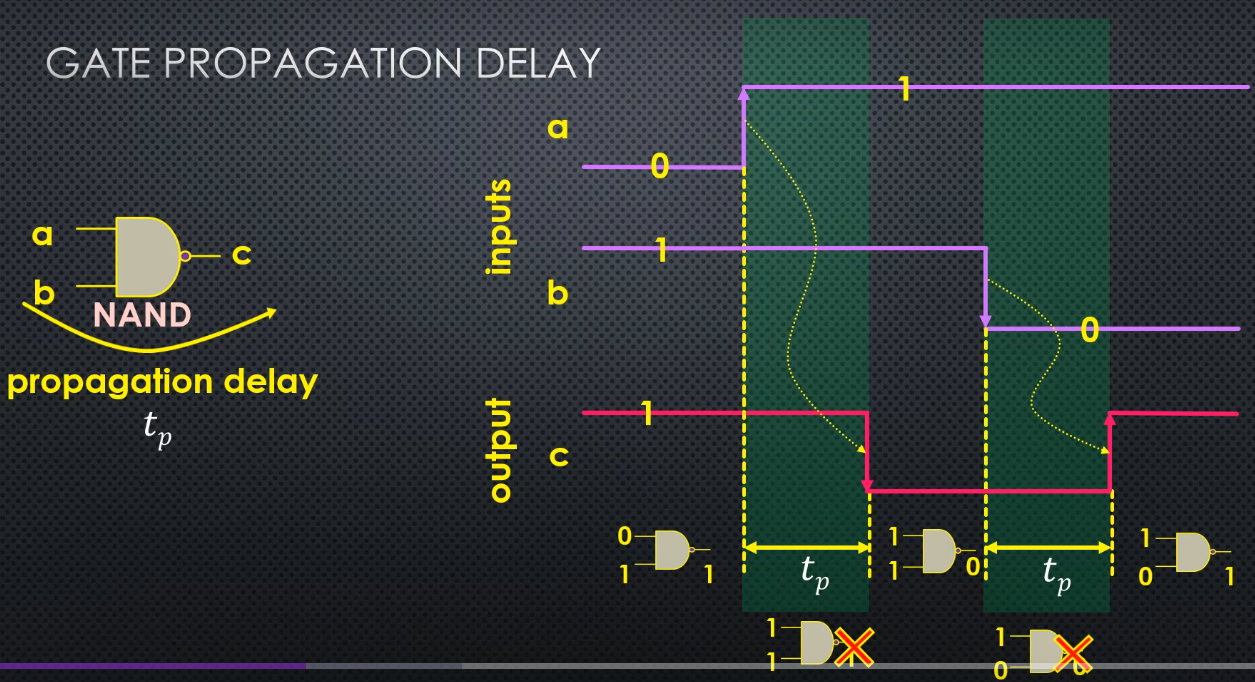
\includegraphics[scale=0.40,frame]{Figures/combinational_circuit/delay_gate_example}
\caption{Propagation Delay Example using NAND gate}
\label{fig:combinational_circuit:delay_gate_example}
\end{figure}

\begin{itemize}

\item When state of $a$ changes from 0 $\rightarrow$ 1, the output didn't appear instantly, it appears after some delay $t_p$

	\begin{itemize}
	\item During this period $t_p$, the output of the NAND gate in invalid and it shouldn't take into accounts
	\end{itemize}

\item Same thing when state of $b$ changes from 1 $\rightarrow$ 0

\end{itemize}

\newpage
The concept of delay also apply to combinational circuit, as it shown in \autoref{fig:combinational_circuit:delay_comb_circuit_example}.

\begin{figure}[h]
\centering
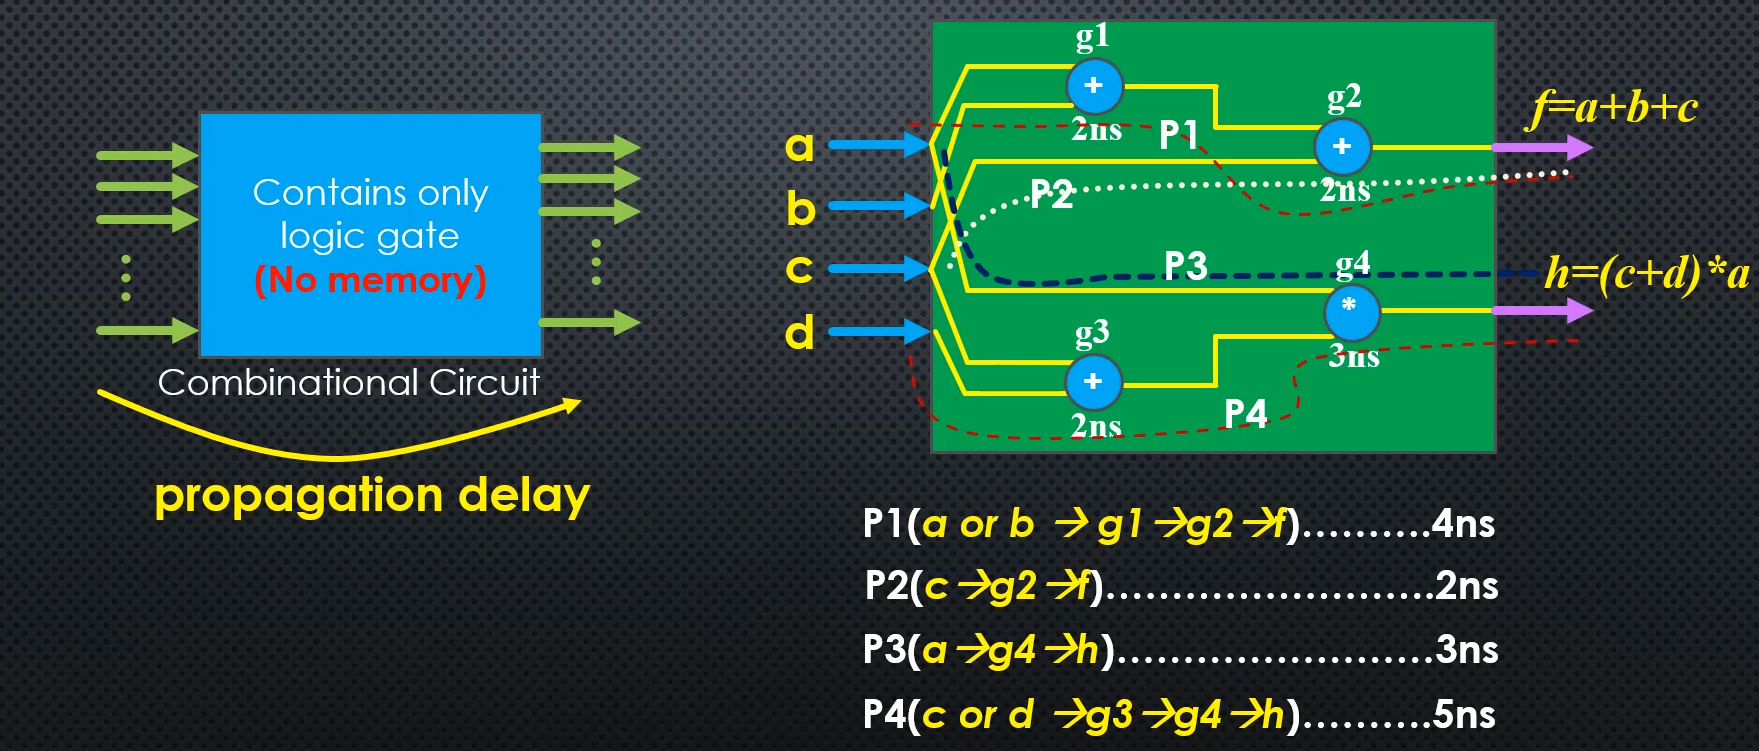
\includegraphics[scale=0.27,frame]{Figures/combinational_circuit/delay_comb_circuit_example}
\caption{Propagation Delay Example in a combinational circuit}
\label{fig:combinational_circuit:delay_comb_circuit_example}
\end{figure}

\begin{itemize}

\item A combinaotional circuit consists of many path, and each path has a certain delay

\item The path with maximum delay is called the \tbi{critical path}

\item we have 4 path $P_i$ and 4 operators $g_i$

\item $P_4$ is the critical path since it has the longest propagation delay

\end{itemize}


In \verb|HLS| desing, \tbi{the goal is to minimize this propagation delay as possible}

\subsection{N Bit Binary Adder}

Let't take an example of computing delay for full binary adder. Its circuit is shown in \autoref{fig:combinational_circuit:full_adder}.

\begin{figure}[h]
\centering
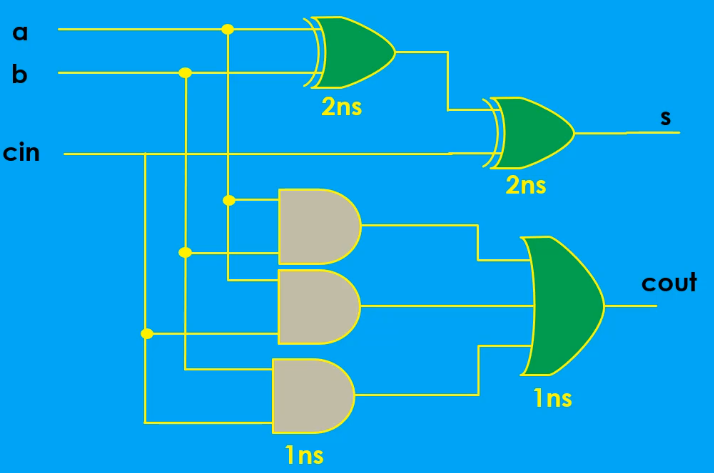
\includegraphics[scale=0.30,frame]{Figures/combinational_circuit/full_adder}
\caption{Full adder circuit}
\label{fig:combinational_circuit:full_adder}
\end{figure}

\newpage
All the path with there delays are shown in \autoref{fig:combinational_circuit:full_adder}.

\begin{figure}[h]
\centering
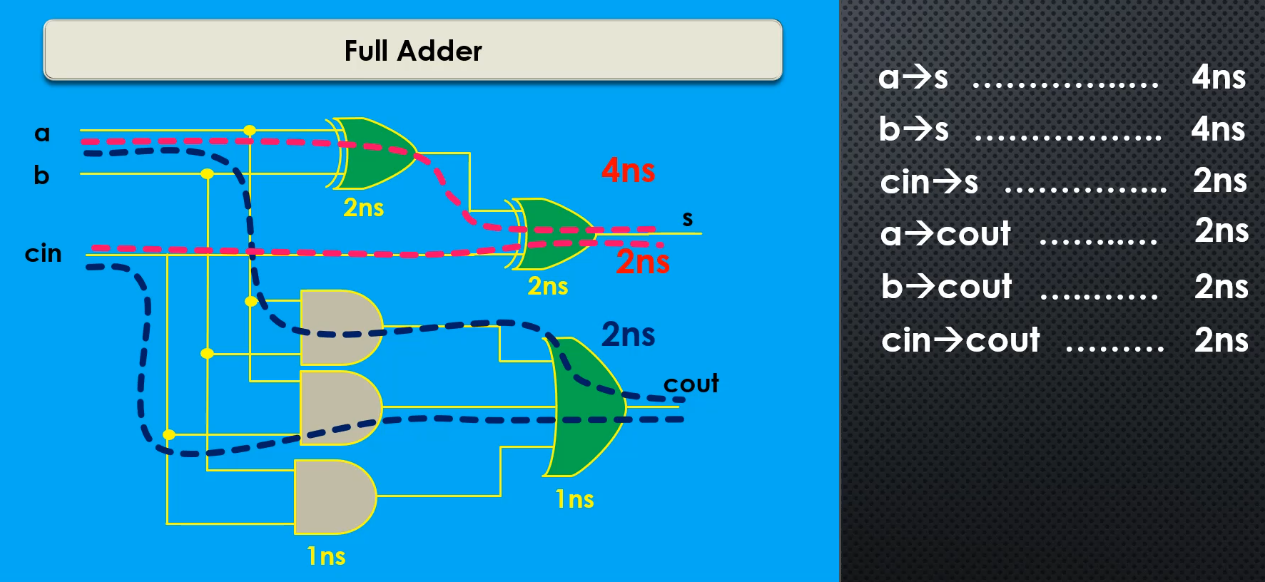
\includegraphics[scale=0.30,frame]{Figures/combinational_circuit/full_adder_delay}
\caption{Delay path for full adder}
\label{fig:combinational_circuit:full_adder_delay}
\end{figure}

So it appears that a full adder output can be used of 4 ns, and any change of the input is not valid till this 4 ns eplases.\\

Now a $N$ bit binary adder can be designed using the \textit{ripple design} shown in \autoref{fig:combinational_circuit:ripple_desing_adder}, where the output carry bit $C_{\text{out}_n}$ is connected to the next adder carry input $C_{\text{in}_{n+1}}$


\begin{figure}[h]
\centering
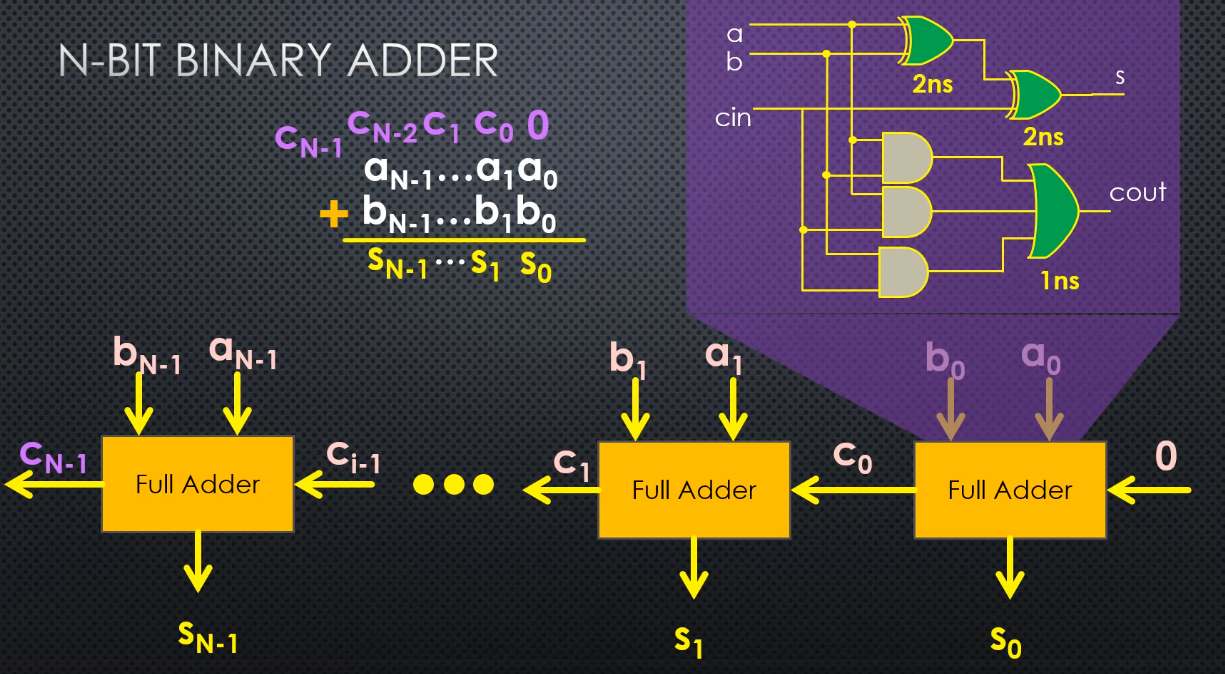
\includegraphics[scale=0.30,frame]{Figures/combinational_circuit/ripple_desing_adder}
\caption{N bit binary adder}
\label{fig:combinational_circuit:ripple_desing_adder}
\end{figure}

\newpage
Each full adder circuit in the $N$ bi adder has 3 path delay shown in  \autoref{fig:combinational_circuit:N_adder_path}

\begin{figure}[h]
\centering
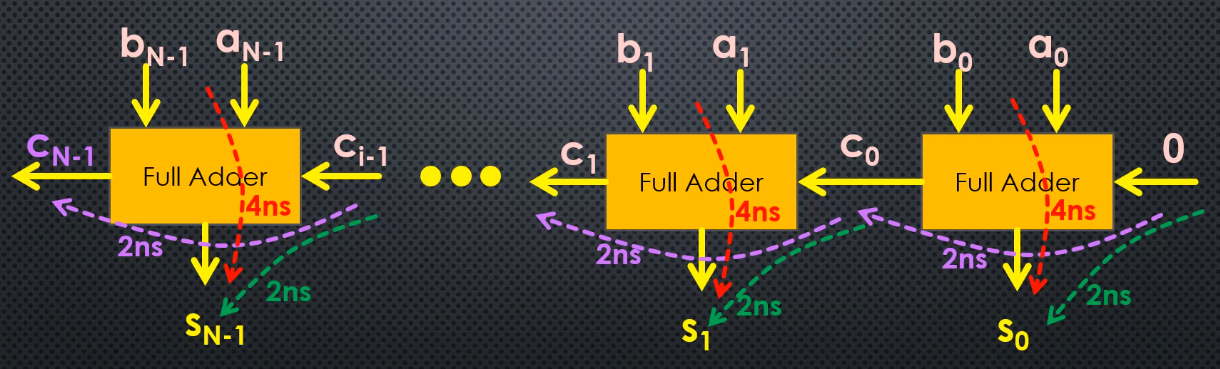
\includegraphics[scale=0.30,frame]{Figures/combinational_circuit/N_adder_path}
\caption{N bit binary adder delay path}
\label{fig:combinational_circuit:N_adder_path}
\end{figure}

\begin{itemize}

\item from $a_n$ and $b_n$ input to $s_n$ output

\item from carry input to sum: $c_{\text{in}_n} \, \longrightarrow \,  s_n$

\item from carry input to carry output: $c_{\text{in}_n} \,  \longrightarrow \,  c_{\text{out}_n}$


\end{itemize}

Now if we want to trace the delay of the $N$ bit adder circuit, we are interested in carry bit and sum bit. Referring back to \autoref{fig:combinational_circuit:full_adder}, the delay from carry input bit to sum bit is 2 ns. The tracing for $N$ bit binary adder is shown in \autoref{fig:combinational_circuit:N_adder_trace_delay}.

\begin{figure}[h]
\centering
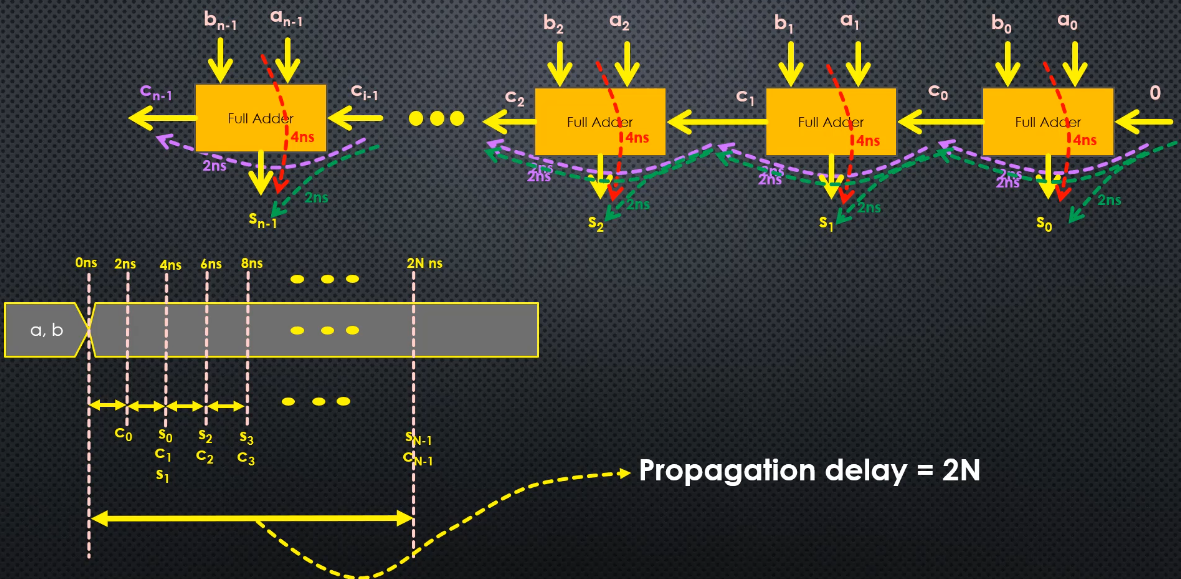
\includegraphics[scale=0.30,frame]{Figures/combinational_circuit/N_adder_trace_delay}
\caption{N bit binary adder: tracing delay}
\label{fig:combinational_circuit:N_adder_trace_delay}
\end{figure}

\begin{itemize}

\item We are assuming that input $a_n$ and  $b_n$ are available at 0 ns

\item Each $n-1$ adder needs 2 ns cycle for the sum and carry bit to be ready

\item We have $N$ adder so the total delay is equal to $2\, N$ ns
\end{itemize}

\newpage
\section{Combinational Circruit in HLS}

Now suppose we have some combinational circuit with some function to represent it, how can we immplement or represent it in \verb|HLS|?

An example is shown in \autoref{fig:combinational_circuit:example_comb_circuit}, where we can represent the function $d$ using 2 types of operators:

\begin{itemize}

\item Bitwise Operator

\item Logical Operator

\end{itemize} 

\begin{figure}[h]
\centering
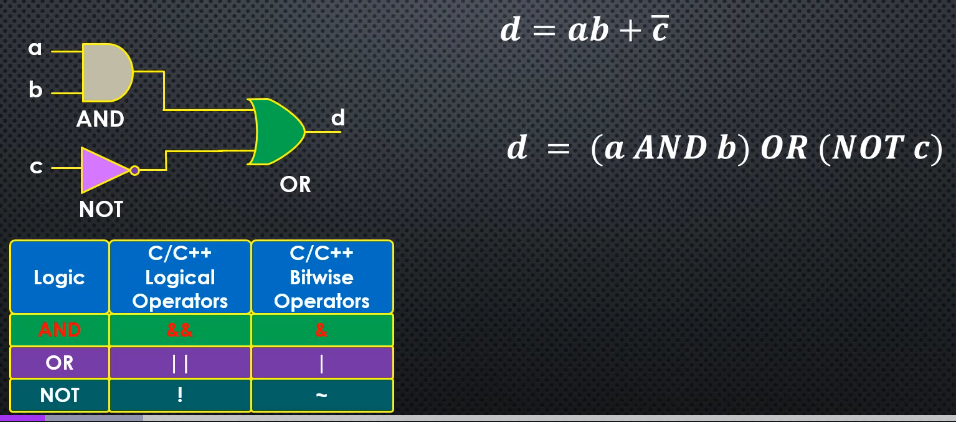
\includegraphics[scale=0.35,frame]{Figures/combinational_circuit/example_comb_circuit}
\caption{Example of a combinational circuit}
\label{fig:combinational_circuit:example_comb_circuit}
\end{figure}

The equivalent \verb|HLS| code is shown in \autoref{fig:combinational_circuit:HLS_comb_circuit}

\begin{figure}[h]
\centering
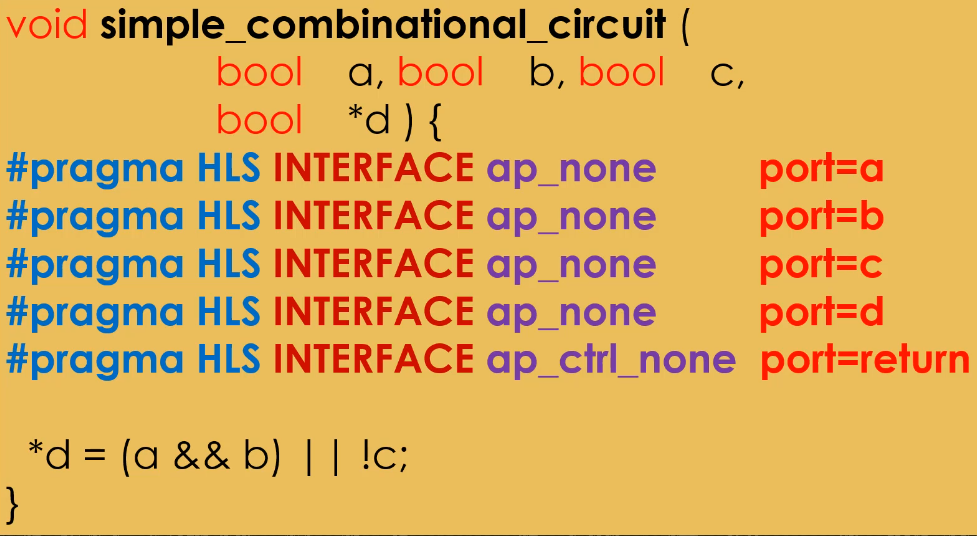
\includegraphics[scale=0.30,frame]{Figures/combinational_circuit/HLS_comb_circuit}
\caption{HLS code for \autoref{fig:combinational_circuit:example_comb_circuit}}
\label{fig:combinational_circuit:HLS_comb_circuit}
\end{figure}

\begin{itemize}

\item Since we are using wires to represent input and output, \verb|ap_none| interface is used for the function arguments

\end{itemize}

\newpage
\subsection{Synthesis Report}

After the function is synthesised using \verb|Vitis|, the report gives us 3 important part, shown in \autoref{fig:combinational_circuit:comb_circuit_report}.


\begin{figure}[h]
\centering
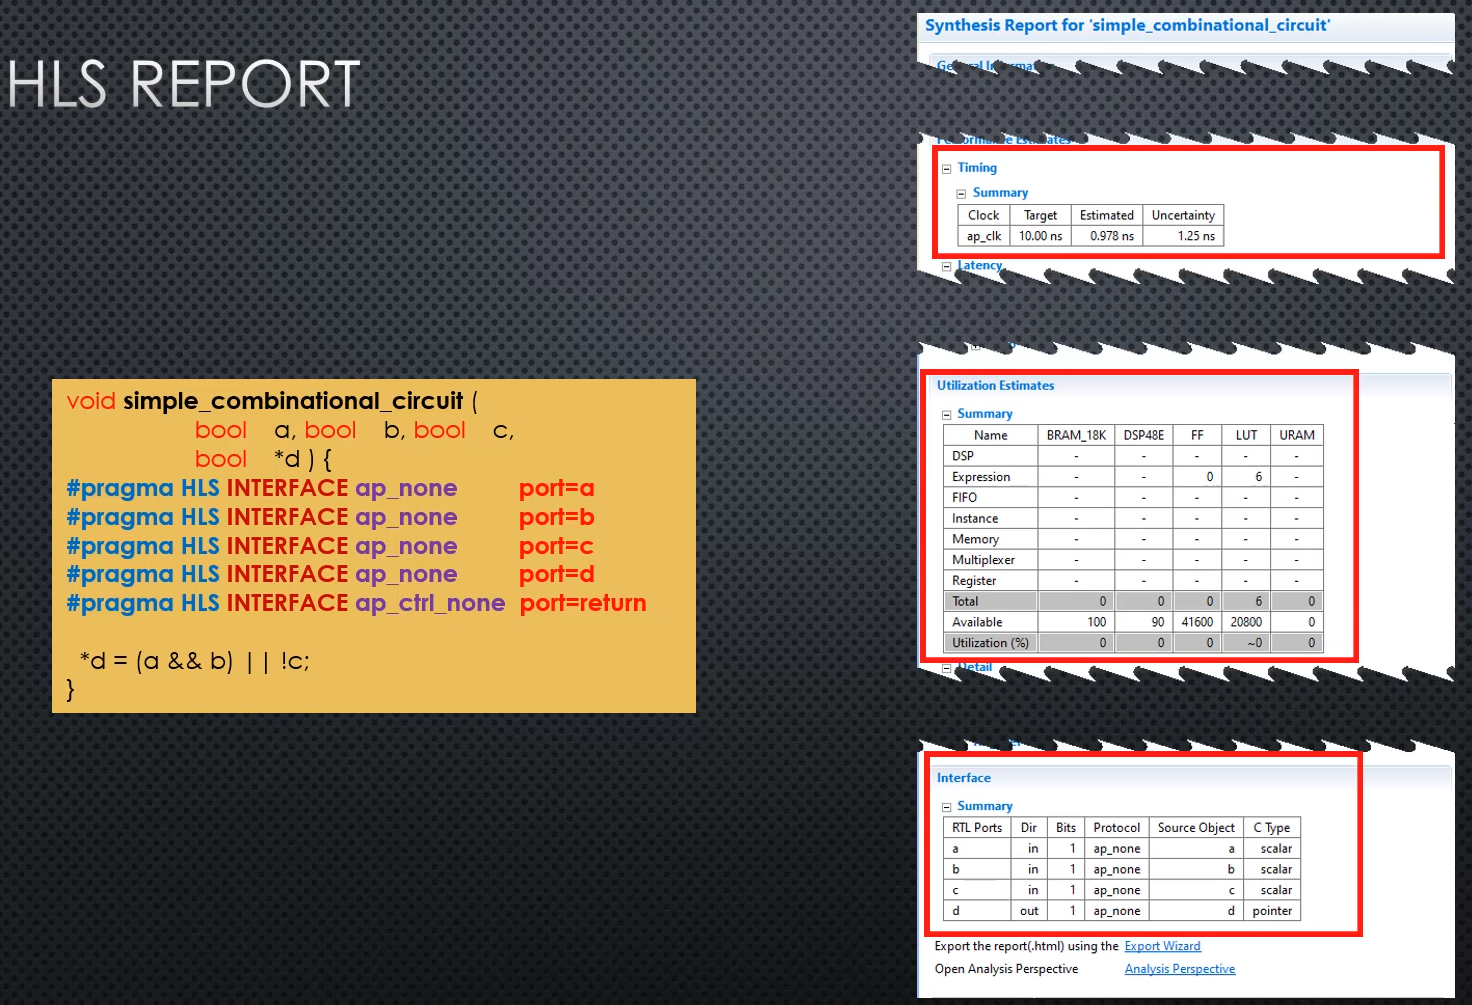
\includegraphics[scale=0.35,frame]{Figures/combinational_circuit/comb_circuit_report}
\caption{Report generation}
\label{fig:combinational_circuit:comb_circuit_report}
\end{figure}

\begin{itemize}

\item Timing part: more for sequential circuit, we skip it for now

	\begin{itemize}
	\item However, we are interested in \textit{estimated} column, where it give us an estimation of $t_p$
	\end{itemize}

\item Resource Utilization: there are the resources we use to synthesize the circuit.

	\begin{itemize}
	\item 3 of the 5 columns are for memory (BRAM,FF,URAM). They should be 0 when dealing with combinational circuit
	
	\item The other 2 are LUT, for logical expression and DSP for mathematical operation, especically for floating point
	\end{itemize}

\item Interface: if for the function arguments part

\end{itemize}


\newpage
\section{Summary}

\begin{itemize}

\item \verb|HLS| desing goal: minimize $t_p$ (\ref{sec:prop_delay})

\item Output of combinational circuit is not valid till $t_p$ elapses

	\begin{itemize}
	\item Also any change of input values, is not valid also till $t_p$ elpases
	\end{itemize}


\end{itemize}



